\documentclass[runningheads]{llncs}
\usepackage[T1]{fontenc}
\usepackage{listings}
\usepackage{graphicx}
\usepackage[inline]{enumitem}
\usepackage{hyperref}
\usepackage[acronym]{glossaries}
\makeglossaries
\newacronym{html}{HTML}{Hypertext Markup Language}
\newacronym{adt}{ADT}{algebraic data type}
\newacronym{dom}{DOM}{Document Object Model}
\newacronym{vdom}{VDOM}{Virtual Document Object Model}
\newacronym{mvu}{MVU}{Model-View-Update}
\newacronym{css}{CSS}{Cascading Style Sheets}
\newacronym{ast}{AST}{abstract syntax tree}
\usepackage{float}
\usepackage{upquote}
\usepackage{fancyvrb}
\usepackage{color}
\definecolor{bluekeywords}{rgb}{0.13,0.13,1}
\definecolor{commentscolor}{rgb}{0.5,0.5,0.5}
\definecolor{greenstrings}{rgb}{0,0.5,0}
\definecolor{codepurple}{rgb}{0.58,0,0.82}
\definecolor{codered}{rgb}{0.8, 0.25, 0.33}
\definecolor{codeorange}{rgb}{1.0, 0.49, 0.0}
\definecolor{codebrown}{rgb}{0.8, 0.58, 0.46}

\lstset{escapeinside={(*@}{@*)}}

\lstdefinelanguage{FSharp}%
{ morekeywords={[0]{let, new, match, with, rec, open, module, namespace, type, of, member, and, for, while, true, false, in, do, begin, end, fun, function, return, yield, try, mutable, if, then, else, cloud, async, static, use, abstract, interface, inherit, finally }},
  otherkeywords={ let!, return!, do!, yield!, use!, var, from, select, where, order, by },
  keywordstyle={[0]{\color{codeorange}}},
  morekeywords={[1]{Value, int, bool, char, string, list, Expr, Env, ADTConstructor}},
  keywordstyle={[1]{\color{codered}}},
  sensitive=true,
  basicstyle=\ttfamily,
  breaklines=true,
  xleftmargin=\parindent,
  aboveskip=\bigskipamount,
  tabsize=2,
  morecomment=[l][\color{greencomments}]{///},
  morecomment=[l][\color{greencomments}]{//},
  morecomment=[s][\color{greencomments}]{{(*}{*)}},
  morestring=[b]",
  showstringspaces=false,
  literate={`}{\`}1,
  stringstyle=\color{redstrings},
  numbers=left,
  stepnumber=1,
}
\definecolor{bluekeywords}{rgb}{0.13,0.13,1}
\definecolor{greencomments}{rgb}{0,0.5,0}

\lstdefinelanguage{JaLi}%
{ keywords={[0]{let, match, with, type, true, false, end, func, function, if, then, else}},
  keywordstyle={[0]\color{codeorange}},
  morekeywords={[1]{Node, String, Tuple, Msg, List, Integer}},
  keywordstyle={[1]{\color{codered}\bfseries}},
  sensitive=true,
  numbers=left,
  stepnumber=1,
  basicstyle=\ttfamily,
  breaklines=true,
  xleftmargin=\parindent,
  aboveskip=\bigskipamount,
  tabsize=2,
  morecomment=[l][\color{commentscolor}]{///},
  morecomment=[l][\color{commentscolor}]{//},
  morecomment=[s][\color{commentscolor}]{{(*}{*)}},
  morestring=[b]',
  showstringspaces=false,
  literate={`}{\`}1,
  stringstyle=\color{greenstrings},
}

\lstdefinelanguage{JavaScript}%
{ keywords={[0]{let, class, const, new, function, if, then, else, super, this, extends, instanceof, return}},
  keywordstyle={[0]\color{codeorange}},
  morekeywords={[1]{Inc, Dec, Increment, Decrement, Message, Node, Tag, Text, Differ, Null, Change, Path, Action, Click}},
  keywordstyle={[1]{\color{codered}\bfseries}},
  sensitive=true,
  numbers=left,
  stepnumber=1,
  basicstyle=\ttfamily,
  breaklines=true,
  xleftmargin=\parindent,
  aboveskip=\bigskipamount,
  tabsize=2,
  morecomment=[l][\color{commentscolor}]{///},
  morecomment=[l][\color{commentscolor}]{//},
  morecomment=[s][\color{commentscolor}]{{(*}{*)}},
  morestring=[b]',
  showstringspaces=false,
  literate={`}{\`}1,
  stringstyle=\color{greenstrings},
}

\lstdefinelanguage{Other}%
{ sensitive=true,
  numbers=left,
  stepnumber=1,
  basicstyle=\ttfamily,
  breaklines=true,
  xleftmargin=\parindent,
  aboveskip=\bigskipamount,
  tabsize=2,
  morecomment=[l][\color{commentscolor}]{///},
  morecomment=[l][\color{commentscolor}]{//},
  morecomment=[s][\color{commentscolor}]{{(*}{*)}},
  morestring=[b]",
  showstringspaces=false,
  literate={`}{\`}1,
  stringstyle=\color{greenstrings},
}
\begin{document}

\title{%  
  Optimization of the model-view-update\break%
  pattern with partial evaluation\break%
}

\author{Liv Hartoft Borre 
\and Jan Schill
}

\authorrunning{L. H. Borre \and J. Schill}

\institute{
IT University of Copenhagen, Copenhagen, Denmark\\
\email{\{livb,schi\}@itu.dk}
}

\maketitle

\begin{abstract}
    Modern techniques to perform DOM updates on rendered HTML documents mostly use a VDOM with comparison of two views, the current view and an updated one after an action is performed. The comparison of tree-structures with subsequent patching of the structure and rerendering is computational expensive. With clever compiler optimizations using partial evaluation these comparisons can be reduced, as the result of an action should always only change in a predictable manner and in the same position in the DOM, hence only a comparison during compile time is needed and thus reduced to a single direct change.
This paper will cover the compiler optimization and the generation of JavaScript snippets, with which the change can be performed, but will not introduce a compiler to JavaScript that would generate a complete working program for the browser.

\end{abstract}

\newcommand{\jan}[1]{\par\smallskip\noindent{\small\llap{\textbf{{jan:}~~}}{\textsf{#1}}}\par\smallskip}
\newcommand{\liv}[1]{\par\smallskip\noindent{\small\llap{\textsf{{liv:}~~}}{\textsl{#1}}}\par\smallskip}
\setcounter{secnumdepth}{-1}
\section{Introduction}\label{introduction}
In order to make websites more dynamic and eliminate the break of the site by loading a new \gls{html} file from the server, many ideas have been shaped and one pattern that solves this problem efficiently is the \gls{mvu} application pattern.
In order to solve the problem of showing diverged information in an \gls{html} document, the JavaScript language needs to be used, as there is no native and complex enough support for \gls{html} or \gls{css} to force the browser to show this new information. JavaScript on the other hand can directly inject into the \gls{dom}, by having complete access to every \gls{html} node element in the rendered \gls{dom}.
JavaScript can select a node element by \texttt{ID} and change its displayed value, forcing the browser to rerender the \gls{dom} on that node. Figure \ref{fig:button_browser} shows a minimal example, where JavaScript is used to alter the rendered \gls{html}.

\begin{figure}
    \centering
    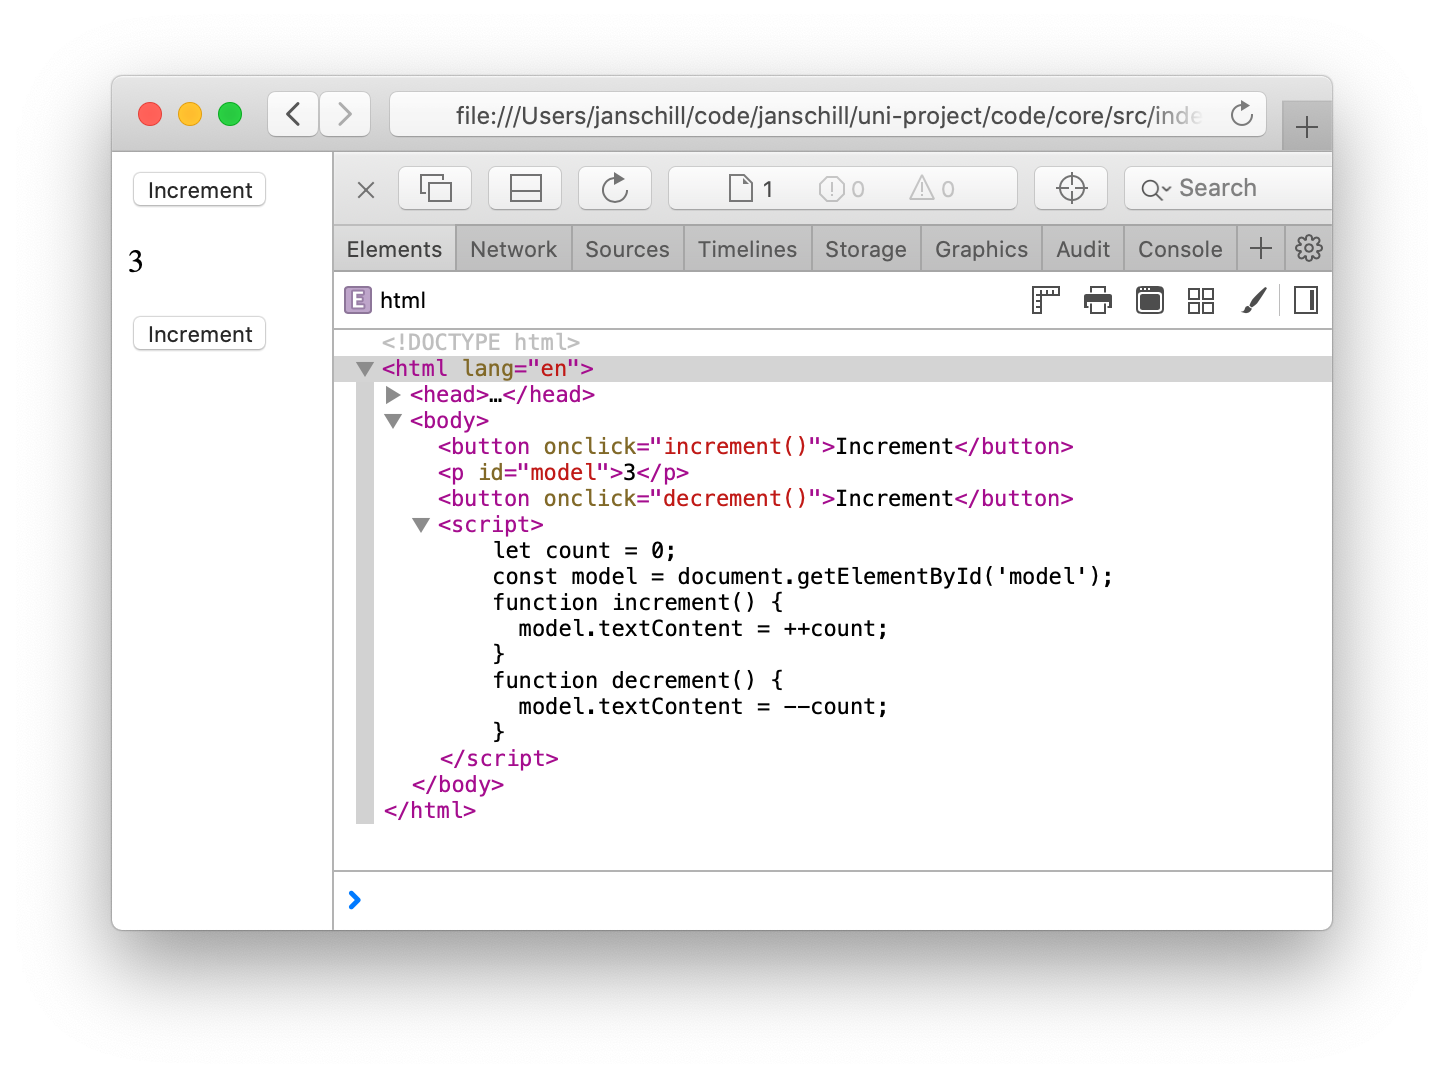
\includegraphics[width=0.8\textwidth]{images/button-browser.png}
    \caption{Simple button counter example}
    \label{fig:button_browser}
\end{figure}

This way of updating content on the document directly has been evolved over the years and is heavily used to build any sized modern websites. With the help of frameworks like React, a JavaScript framework developed by Facebook or Elm a framework that uses its own functional language, it has become easier to go from a small button example to a fully working componentized website.
The Elm framework uses the \gls{mvu} application pattern to realize the idea of dynamically updating the \gls{dom}.

The basic functionality how Elm uses it, is that it generates \gls{html} that can be viewed by a client. This client can then interact with the \gls{html} by clicking a button for example, producing a \texttt{Msg (Message)}, which is send to Elm, producing another \gls{html} document.
In the Elm program three parts play a crucial role: the Model, View and Update.

When a message of type \texttt{Msg} is produced, the update function is being called, which takes the message sent and the current state of the model, returning an updated model. The view function, responsible of generating the \gls{html} that can be views by the browser is called automatically, rendering the \gls{html} with the updated model.

\begin{verbatim}
view : Model -> Html Msg
update : Msg -> Model -> Model
\end{verbatim}

\paragraph{How does Elm optimise the view rendering?}
Because most of the time when a new view was generated and needs re-rendered, it is not necessary for the whole document to be switched out, but rather only the \gls{dom} node that experienced change -- forcing the browser to generate new \gls{dom} nodes is computational expensive work.
For this most frameworks use a \gls{vdom}, which resembles the complete active \gls{dom} in memory in a convenient data structure. This \gls{vdom} is then generated with the updated model and compared against the current active \gls{vdom}, finding the parts that need updating. This part is called \textit{diffing} and it is done by iterating over both representations of the \gls{dom} and comparing each individual node. This \textit{diffing} then generates a data structure that keeps track of all changes. A \textit{patch} function, taking the old view and the data structure holding the changes, then generates a representation of the new view by switching out all the nodes that need updating.

All the \textit{diffing} and \textit{patching} against the whole \gls{dom} tree seems to be still computational expensive, when in the end for the button example only the following is needed:

\begin{figure}[]
    \centering
\begin{verbatim}
<html>
  <button onclick=increment()>Increment</button>
  <p id="model">0</p>
</html>
<script>
  let count = 0;
  const model = document.getElementById('model');
  function increment() {
    model.textContent = ++count;
  }
</script>
\end{verbatim}
    \caption{Reduced example to show only the incrementing}
    \label{fig:button-increment}
\end{figure}

\paragraph{How does JaLi optimize the view rendering even further?} This paper will outline all the needed parts to use partial evaluation, symbolic execution and constant folding to optimize the view rendering. It will be shown on the small button example how the compiler of the JaLi language can reduce all the previously mentioned parts that are computational expensive, by applying the optimizations.
Due to time restrictions it was not able to implement the full working compiler optimizations, nor a compiler that transforms a full program to a \gls{html} and JavaScript website that could be run in the browser. Nevertheless the theory has been established and it will be shown on small examples to illustrate the idea.
\newpage
\setcounter{secnumdepth}{2}
\section{The JaLi language} \label{jali}
The JaLi language is a minimal higher-order functional language without type checking. The syntax is closely coupled to FSharp and Haskell.

\lstinputlisting[label={jali_button_example}, language=JaLi, caption=Button example written in JaLi]{./code/button.jali}
    
Listing \ref{jali_button_example} shows how the button example from the previous chapter could look like in the JaLi language.
It introduces an \gls{adt} called \texttt{Node} in line 1, that has two constructors: \texttt{Text} and \texttt{Tag}. An \gls{adt} is a composition type, which means that it is used to introduce new and more complex types to a language. This is especially useful when wanting to depict a type from the outside into the language. To illustrate this on an example by also continuing to explain the given example:
The \texttt{Node} type is representing an \gls{html} document element. In \gls{html} an element always carries an element name, for example \texttt{button}: \texttt{<button></button>}; a list of key-value pairs, named as \gls{attributes}: \texttt{id=buttonIncrement} , which are set after the element name in the opening tag and lastly it holds elements or text in between its opening and closing tags.

\begin{lstlisting}[columns=fullflexible, label={button_increment_html}, language=JaLi, caption=Button increment in HTML]
<button id=buttonIncrement>Increment</button>
\end{lstlisting}

Represented in JaLi as an \gls{adt} the single button \gls{html} element would look like in listing \ref{button_increment_jali}.

\begin{lstlisting}[columns=fullflexible, label={button_increment_jali}, language=JaLi, caption=Button increment in JaLi as ADT]
Tag ('button') ([('id', 'buttonIncrement')]) ([
  Text 'Increment'
])
\end{lstlisting}

Just like in \gls{html} then, the \gls{adt} can recursively be nested to construct a tree-like structure.
Another example for this would be a recursive list data type

\begin{lstlisting}[columns=fullflexible, label={recursive_list}, language=JaLi, caption=Recursive list data type]
type List = Nil | Cons Integer List;

Cons 1 (Cons 2 (Cons 3 (Nil)))
\end{lstlisting}

An \gls{adt} always carries super-type defined right after the keyword \texttt{type}, followed by a number of constructors, which are used to instantiate an actual value of the defined \gls{adt}. These constructors can carry optional type parameters, which need to be given, when creating it. Like in the listing \ref{button_increment_jali} the \texttt{Tag} constructor needs a string and two lists.

\glspl{adt} make mostly only sense with pattern matching implemented as well. Pattern matching will allow the flow of the program according to the state of the matching \gls{adt} values.

\begin{lstlisting}[columns=fullflexible, label={pattern_match}, language=JaLi, caption=Pattern matching on Msg]
type Msg = Increment | Decrement;
message = Increment;

match message with
  | Increment -> 'Increment the model'
  | Decrement -> 'Decrement the model'
  | _ -> 'Unknown action'
\end{lstlisting}

The example in listing \ref{pattern_match} shows the known \gls{adt} definition in line 1. After it on line 2 a \textit{let binding} can be seen, where the value on the right side is assigned to the variable called \texttt{message}. Afterwards this binding is used in pattern matching context. The value of \texttt{message} will be matched with the available patterns defined after the pipe symbol. There are three patterns that can be matched with, each valid action and one \textit{wild card} pattern, that acts like the \textit{else} block in an \textit{if statement}. The complete \texttt{match} block will then return only the right side of the matched pattern.

Functions are defined by enclosing a name, parameters and a function body between the key words \texttt{func} and \texttt{end}.

\begin{lstlisting}[columns=fullflexible, label={pattern_match}, language=JaLi, caption=Pattern matching on Msg]
func factorial n =
  func mult x y =
    x * y
  end
  
  if n == 0
  then 1
  else mult (n) (factorial (n - 1))
end
factorial 5 // => 120
\end{lstlisting}

Functions can be recursively called and can even have inner functions.

\subsection{Grammar}\label{Grammar}
The lexer, parser and interpreter are all written in FSharp with the help of the libraries \textit{FsLex} and \textit{FsYacc}.

\subsubsection{Lexer}
The lexer receives a JaLi program as a string, recognizes and transforms its characters in the program to tokens in FSharp. These tokens are defined in the \textit{Lexer.fsl} and \textit{Parser.fsy}. The lexer does this by having a defined list of regular expressions to tokens and matches the input string character by character to those patterns.
The result is a list of tokens that might end up looking lik listing \ref{lexer_input}

\begin{lstlisting}[columns=fullflexible, label={lexer_input}, language=JaLi, caption=Lexer result]
// JaLi program as string:
"5 + 10"
// Result of lexing the string:
Parser.token = CONSTINT 5
Parser.token = PLUS
Parser.token = CONSTINT 10
Parser.token = EOF
\end{lstlisting}

After the whole string is successfully transformed into tokens, the parser will try to make sense of it.

\subsubsection{Parser}
The parser receives the list of tokens after the lexical analysis and builds an \gls{ast} from it. It does this by recognizing different combinations of tokens, that are defined explicitly.

In the case of JaLi, a program -- indicated by is point of entry with \texttt{Main} -- is an \texttt{Expression}, which is defined in the parser as the following:

\begin{lstlisting}[columns=fullflexible, label={parser_expression}, language=FSharp, caption=Program defined by \texttt{Expression}]
Main:
    Expression EOF { $1 }

Expression:
  | AtomicExpression { $1 }
  | FunctionCall { $1 }
  | ConditionalExpression { $1 }
  | Baseoperation { $1 }
  | Binding { $1 }
\end{lstlisting}

From only knowing this, it might not be obvious how a program then can be multiple \texttt{Bindings} or \texttt{Functions} with a \texttt{FunctionCall} in the end. This is realized by defining a \texttt{Binding} by its \texttt{Expression} that it binds to, but also expecting another \texttt{Expression} right after the binding.

\begin{lstlisting}[columns=fullflexible, label={parser_binding}, language=FSharp, caption=Binding with \texttt{Expression} afterwards]
Binding:
  | LocalBinding { $1 }
  | FunctionBinding { $1 }
  | ADTBinding { $1 }
  
LocalBinding:
  | NAME ASSIGN Expression SEMICOLON Expression { Let($1, $3, $5) }
\end{lstlisting}

The \texttt{SEMICOLON} marks an end of a \texttt{Binding}, indicating that the \texttt{Expression} after it, is the next \texttt{Expression} in the program -- allowing multi-line programs and not just a single line program. The part in curly braces after a parser rule was up until here completely ignored, but shall be explained as being the mapping to its \gls{ast} element. A \texttt{Binding} in the \gls{ast} is represented by a \texttt{Let} key word, which holds three values, these are passed over by the call on line 7 in listing \ref{parser_binding}.
The \texttt{Let} is specified as \texttt{Let of string * Expr * Expr} in the \gls{ast} file. This means that the first parameter needs to be of type string, the name and the other two parameters of type \texttt{Expr}, which is a defined type.

\begin{lstlisting}[columns=fullflexible, label={ast}, language=FSharp, caption=An excerpt of the \gls{ast} of JaLi]
type Value =    
    | IntegerValue of int
    | BooleanValue of bool
    | CharValue of char
    | StringValue of string
    | TupleValue of Value * Value
    | ListValue of Value list
    | ADTValue of string * string * Value list
    | Closure of string * string list * Expr * Value Env
    | ADTClosure of ADTConstructor * string * Value Env

and Expr =
    | ConcatC of Expr * Expr
    | List of Expr list
    | Constant of Value
    | StringLiteral of string
    | Variable of string
    | Tuple of Expr * Expr
    | Prim of string * Expr * Expr
    | Let of string * Expr * Expr
    | If of Expr * Expr * Expr
    | Function of string * string list * Expr * Expr
    | ADT of string * ADTConstructor list * Expr
    | Apply of Expr * Expr list
    | Pattern of Expr * (Expr * Expr) list
\end{lstlisting}

\vspace{0.3cm}

The listing \ref{ast} gives a rough overview of the multiple \texttt{Expressions} that are currently implemented and reveal a bit of its possibilities.

Returning back to the grammar in the parser the implementation and characteristic of the JaLi grammar shall be explained.
As already mentioned everything reduces to an \texttt{Expression}, which are split into the ones shown in listing \ref{parser_expression}.

We distinguish between \texttt{Atomic Expression} and other expressions. An \texttt{Atomic Expression} is a constant, a variable, a tuple, a list, a cons operator, or a parenthesized expression (so that it is easy to see where an \texttt{Atomic Expression} begins and ends). Constants are integers, booleans, strings, and the wildcard character '\_' which is used for match expressions.

The reason we make this distinction is because syntax like function applications without parentheses makes the language ambiguous, as we then can not decide when the function application expression ends and another begins. A solution to this, is to distinguish between \texttt{Atomic Expression} and other expressions, and then require arguments for function application to be atomic. 
\\\\
Besides \texttt{Atomic Expression}, an expression can be a logical negation, a base operation for arithmetic and comparison (+, -, ==), a conditional expressions, a match expressions, a function call or a binding. A binding is an \gls{adt} declaration, a local binding, or a function declaration. 

\begin{Verbatim}[numbers=left,xleftmargin=\parindent]
Main ::=
  expr

expr ::=
  atomicexpr                            atomic expression
  !expr                                 logical negation
  expr op expr                          base operations, arithmetic, 
                                        comparison
  if expr then expr else expr           conditional expression
  match expr with patterns              match expression
  NAME atomicexprs                      function call
  binding                               types, locals, functions

atomicexpr ::=
  const                                 constant literals
  NAME                                  local variable or parameter
  (expr, expr)                          tuple
  [ expr, expr, ..., expr ]             list
  expr::expr                            cons operator
  ( expr )                              parenthesized expression

const ::=
  CONSTINT                              integer literal
  CONSTBOOL                             boolean literal
  STRINGLITERAL                         string literal
  USCORE                                wildcard literal

binding ::=
  type NAME = constructors; expr        abstract data type binding
  NAME = expr; expr                     local binding
  function NAME params = expr end expr  function binding

patterns ::=
  | expr -> expr                        one pattern
  | expr -> expr patterns               more than one pattern

constructors ::=
  NAME typeparams                       one type constructor
  NAME typeparams | constructors        more than one type constructor

type ::=
  INT                                   Integer type
  FLOAT                                 Float type
  BOOLEAN                               Boolean type
  STRING                                String type
  CHAR                                  Char type
  NAME                                  Name variable type
  ( type, type )                        Tuple of types
  [ type ]                              List of type
  
typeparams ::=
  (* empty *)                           zero type parameters
  type typeparams                       more than zero type parameters

atomicexprs ::=
  atomicexpr                            one expression
  atomicexpr atomicexprs                more than one expression

params ::=
  NAME                                  one parameter
  NAME params
\end{Verbatim}


\newpage

\section{Reducer}\label{reducer}
The essence of what we are going to do is that we are going to exploit as much of the statically known data in the program, by reducing it into a smaller residual program, which is then compiled into \gls{html} and JavaScript. The program we are reducing is the \gls{mvu} described in the introduction \ref{introduction}. Reducing this program will allow us to optimize the entire diffing cycle, because we can generate JavaScript functions that know exactly what document elements to change, when called. This is all to achieve improved efficiency compared to current \gls{vdom} diffing. However, in order to understand and apply it, partial evaluation needs to be understood.

\subsection{Partial evaluation}
When all inputs to a program are given, an interpreter evaluates the program, and obtains a result. However, this is possible only when all of the inputs are known. 
Partial evaluation is a program optimization technique concerned with specialization and evaluation of programs where only parts of the inputs are known. 
\\\\
Most developers are familiar with specialization from partial application of functions. Partially applying a two-argument function obtains a one argument function where the first value has been \textit{fixed} to the given value. Fixing the variable to a specific value is called specialization. 
\\\\
A partial evaluator is an algorithm which, when given a program and some of its input, will attempt to execute the program as far as possible, and output a reduced \textit{residual} program. When given the remaining inputs the residual program will execute the rest of the program. It works as if the input has been \textit{incorporated} into the original program, as much as possible has been evaluated, and unnecessary branches have been reduced away. Evaluation of the residual program with the remainder of the inputs should yield the same output as evaluation of the original program with all of the inputs. In that sense, it is a specialized version of the original program. Partial evaluation is also known as \textit{program specialization}.
\\\\
The below Figure \ref{specialize-easy} is an example from \cite{Sestoft} showing a two-input program p for computing $x^n$. Partially evaluating the program with the static parameter 5 yields the second specialized program p5.

\begin{lstlisting}[columns=fullflexible, label={specialize-easy}, language=Other, caption={Specialization of a program to compute $x^n$}]
f(n,x) =
  if n = 0 then 1
  else if even(n) then f(n/2,x)^2
  else x * f(n-1,x)

f5(x) = x * ((x^2)^2)
\end{lstlisting}

The reason why this is beneficial is for efficiency gains. Partially evaluating the program with 5 yields the program \texttt{p5} where this expensive computation has already been done. Thus \texttt{p5(x)} is a much faster program than \texttt{p(5)(x)}. It is worth to note that this optimization is possible because n determines the control of the program. If \texttt{x} was the static parameter, it would not be possible to achieve the same optimization. 
\\\\
Figure \ref{specialize-update} shows another example, of the two-input function \texttt{update}, which either increments or decrements the model by one, based on the given \texttt{msg}. Partially evaluating the function with the static parameter \texttt{Increment} yields a new function which always adds 1 to the model it receives. 

\begin{lstlisting}[columns=fullflexible, label={specialize-update}, language=JaLi, caption={Specialization of the update function on increment}]
func update msg model =
  match msg with
  | Increment -> model + 1
  | Decrement -> model - 1
end

func updateIncrement model =
  model + 1
end
\end{lstlisting}

Let's assume that each branch contains some expensive computation. Partially evaluating \texttt{update} with \texttt{Increment} yields the function \texttt{updateIncrement} where this expensive computation has already been done. This is desirable when the function is called with several different second parameters, as it allows to reuse \texttt{updateIncrement} with several different arguments without recomputing the expensive computation. Thus efficiency can be achieved by partially evaluating the \texttt{update} function with each of the inputs \texttt{Decrement} and \texttt{Increment}, and replace all calls to \texttt{update(Increment)} with the specialized function \texttt{updateIncrement}, and replace all calls to \texttt{update(Decrement)} with the reduced function \texttt{updateDecrement}.

\subsection{Approach}
So what is actually going on in partial evaluation, is a combination of evaluation and code generation. We are evaluating all calculations that depend only on the known input. These expressions are called \textit{static}. All expressions that rely on unknown inputs are called \textit{dynamic}. For each dynamic expression we generate code by replacing it with a new expression. This is described by the following techniques. 
%\liv {Currently we are reducing expressions away, e.g. when %reducing Function(..), but maybe we shouldn't?: '\textit{In %general, reduction of the static version (at specialization %time) will produce a value, whereas reduction of the dynamic %version will not change its form, only reduce its %subexpressions}'.)}
There are three main techniques in partial evaluation \cite{Sestoft}: \textit{symbolic computation}, \textit{unfolding function calls}, and \textit{program point specialization}. The two first techniques have been sufficient for this project and will be described here, while the third one will be described in improvements.
\paragraph{Symbolic computation:} This is the process of computing with symbolic values either by rewriting or evaluation. Symbols, in this context expression, represent rewritable terms, while values imply the end of rewritability. We are going to specialize function bodies by reducing it symbolically; we will rewrite dynamic expressions to other expressions (code generation) and evaluate static expression into values.
\paragraph{Unfolding:} This means replacing a function call by a copy of \texttt{f's} body where all parameter variables have been replaced by the corresponding arguments. E.g. if there is somewhere in the program that the partial evaluator finds a call to \texttt{unfold Increment 5} it will replace the call with the constant 6.
\paragraph{Unfolding Strategy:} Unfolding can either be done \textit{on the fly} or in a post phase. We will be using the former. To avoid infinite unfolding, Sestoft \cite{Sestoft} proposes three strategies.
\begin{enumerate}
    \item Avoid infinite unfolding by not unfolding function calls, however this would mean that the function calls would not be unfolded even though the arguments are static, resulting in a minimal specialization.
    \item Only unfold function calls when all parameters are static. This risks only infinite unfolding if the original program had a potential \textit{infinite static loop}, i.e. a loop that does not involve any dynamic tests.
    \item Not to unfold a function call inside a dynamic conditional. As before, this avoids infinite unfolding as long as the original program does not contain a potential infinite static loop itself.
\end{enumerate}

We will be using the latter strategy, however since the control flow in our language is also determined by pattern matching, we will extend the constraint to also apply in dynamic match expressions. 

\paragraph{Offline and online partial evaluation:}
One should note that there are two different processes for partial evaluation: online and offline. Offline divides the partial evaluation into two stages. The first is a preprocessing phase, where expressions are divided in static and dynamic expressions, e.g. by annotating each expression as either dynamic or static, based on the available information. Then during the actual specialization, the decision of whether a certain expression should be reduced or not is based on the precomputed division. Online processing consists of only one phase: the action to take at each expression is decided based on the concrete values computed during specialization. The main advantage of the online process is that it exploits more static information during specialization than the offline process \cite{Sestoft}. The online process will be followed.

%** Sestoft book ** 
%- pre-compute all expressions involving n
%- unfold the recursive calls to function f
%- reduce x*1 to x.

%- Partial evaluation can even be advantageous in a \textit{single run}, since it often happens that partial evaluation p on in1 and then running on in2, is faster than running p on in1 and in2. An analogy is that compilation plus target run time is often faster than interpretation in Lisp.

% Does partial evaluation eliminate the need to write compilers? Yes and no...Pro: ... Contra: the generated target code is in the partial evaluator's output language, typically the language the interpreter is written in. ... 

%** Sestoft book end **

\subsection{Implementation}
Our partial evaluator is going to produce a residual program by running through the program and pre-compute as much as possible, based on static variables and arguments to function calls. Having detailed the expressions of the JaLi language in Chapter 3, here it will be explain how each of them are reduced by the partial evalutor. 
\\\\
\textit{A note on the implementation}: The reduction of the expressions is mostly trivial, however reducing the patterns are quite complex. We believe that this is mainly caused by the abstract syntax behind JaLi, mainly in the different representations of \glspl{adt}. A much simpler implementation of the reducer is very likely, with a better implementation of the abstract syntax. Another notable thing is that this is not an optimal implementation of the reducer, as it may reduce function bodies and other expressions even though no static information is available and thus no reduction will be achieved. For now, this works just fine for the examples demonstrated.
\\\\
The partial evaluator is implemented as the single function \texttt{reduce} as seen in listing \ref{reduce-base}. As main parameters it takes an expression to reduce and a store. The store is a list of variable bindings similar to the environment parameter in the interpreter; it is a list of (string, Expr) tuples, mapping a name to an expression. The last parameter is the \textit{context} which expresses whether it is inside a dynamic conditional. This is to implement the unfolding strategy that does not unfold function calls inside dynamic conditionals. When done, the reduce function outputs an Expr.
\\\\
Reducing a constant returns the constant. Reducing a variable will look up the variable in the store and return the expression. 

\lstinputlisting[columns=fullflexible, label={reduce-base}, language=JaLi, caption=The reduce function]{./code/compiler/base.jali}

Listing \ref{reduce-ctl} shows the reduction of concatenations, tuples and lists, as these cases resemble each other. We reduce each of the sub-expressions. For concatenation and lists we return a list and for tuples we return a tuple with the reduced sub-expressions.

\lstinputlisting[columns=fullflexible, label={reduce-ctl}, language=JaLi, caption=Reducing concatenations tuples and lists operations]{./code/compiler/concat-tuple-list.jali}

As shown in listing \ref{reduce-prim}, a primitive operation is reduced similarly to the previous, by reducing each sub-expression. If both are constant, the interpreter will be used to evaluate the primitive expression and return a constant value. However, even though one of the sub-expressions are not constant, it may still be possible to reduce the expression. E.g. multiplying a variable with 0 will always yield zero, as seen in the match cases in the listing. For the problems that are being showcased, it suffices to consider only these cases. However, the list is not exhaustive, and a complete partial evaluator should consider many more cases in order to be optimal.

\lstinputlisting[columns=fullflexible, label={reduce-prim}, language=JaLi, caption=Reducing primitive operations]{./code/compiler/prim.jali}

Listing \ref{reduce-let} shows reduction of let-bindings. When reducing let-expressions the body will be reduced first. Then the result will be added to the store, bound to the name of the binding variable. Lastly the following expression will be reduced. This effectively removes the let binding expressions. The expression lives in the store and replaces dynamic variables at the places where it is referenced.

\lstinputlisting[columns=fullflexible, label={reduce-let}, language=JaLi, caption=Reducing let bindings]{./code/compiler/let.jali}

Reducing conditionals is shown in listing \ref{reduce-cond}. First, the conditional expression is reduced. If the expression is a constant boolean value, we already know what branch the program will take, and thus we return the reduction of this branch. If the conditional is not a constant, we return a conditional expression with the branches reduced. As according to our unfolding strategy, we change the context to false, expressing that we are inside a dynamic conditional, and thus should not unfold function calls when encountering them.

\lstinputlisting[columns=fullflexible, label={reduce-cond}, language=JaLi, caption=Reducing conditional expressions]{./code/compiler/cond.jali}

Listing \ref{reduce-function} shows the reduction of functions. In order to handle recursive calls, we add the closure to the store before reducing the function body. Then we create a new closure with the reduced body, add it to the original store, and continue by reducing the second expression that follows the function. Here we always return the reduced expression that follows the function. The function exists as a closure in the store, which will be specialized and unfolded at function calls.

\lstinputlisting[columns=fullflexible, label={reduce-function}, language=JaLi, caption=Reducing functions]{./code/compiler/function.jali}

Reducing \gls{adt} definitions happens in listing \ref{reduce-adt} by adding the constructors to the store and continue reducing the following expression. If the constructor has no parameters, it is an \gls{adt} value and otherwise an \gls{adt} constructor. A simpler representation of \gls{adt} constructors would be desirable, as the differences causes complexity in the patterns matching.

\lstinputlisting[columns=fullflexible, label={reduce-adt}, language=JaLi, caption=Reducing \gls{adt} declarations]{./code/compiler/ADT.jali}

Function application in listing \ref{reduce-apply} are reduced by first reducing the expression to apply and the arguments given. The reduced expression may either be a closure, \gls{adt} closure or a constant. When reducing a closure, we check if the context is true, meaning that are not in a dynamic conditional, and thus may unfold function calls. That is, we replace the function application with the specialized function body of the closure. If the context is false, we do not unfold the function body, but rather return and apply the expression. This results in not being able to handle partial function application, which is no problem as this suffices for the examples at hand. If the closure is an \gls{adt} closure, we check if all required arguments are given. If the arguments are all static, we return a constant \gls{adt} value, and otherwise return an \texttt{Apply} to the \gls{adt} closure. 

\lstinputlisting[columns=fullflexible, label={reduce-apply}, language=JaLi, caption={Reducing function application}]{./code/compiler/apply.jali}

The complexity of the reducer lays in the reduction of patterns. The reduction of patterns is given in listing \ref{reduce-pattern}, but which utilizes the \texttt{match1} function given in listing \ref{reduce-util}. The \texttt{match1} will try to match a single pattern with the match expression. When a pattern contains a variable name, it is a binding of an expression to a name, which shall be used in the body of the patterns. Thus, this is the main task of the \texttt{match1} function: Try to match a value with a given pattern and collect all the bindings in the pattern. This is the complex and main part of this reduction. A matching is represented by the type \texttt{ReducedMatch}, which can take three different forms. Either it is a \texttt{NoMatch}, if it is certain that the pattern will never match, even when the dynamic variables of the match expression is known. A \texttt{DynamicMatch} means that the pattern could possibly match, once the dynamic variables are known. The \texttt{StaticMatch} is certain that the pattern will match. Dynamic and static matches carry a list of bindings, which is a list of tuples of name and expression. 
\\\\
The \texttt{matchMany} function is a helper function for when many expressions determines whether a match is static or dynamic or a no match - e.g. in lists. The function matches all expressions in the list, and checks if one of them is a \texttt{NoMatch}. Otherwise it collects all the bindings that result from the matching. If any of them is dynamic, then the entire result is a dynamic match, and otherwise it is static. 
\\\\
The last helper function is \texttt{collect} which simply traverses the pattern and collects all variables as bindings to itself. This is used when the match expression is itself a dynamic variable. Then we cannot match any further in the pattern, but we still need to collect the rest of the bindings from the pattern in order to reduce the body.
\\\\
Returning back to the reduce function in listing \ref{reduce-pattern}. First the match expression is reduced, and the result is either a constant or it is dynamic. In either case we need to match the expression with the given patterns and reduce the body of the pattern. If the match expression is constant, we know that one of the patterns must match statically. Thus, we just need to find the first static match. The bindings are then added to the store, before reducing the body of the pattern and returning the reduced expression.
\\\\
If the match expression is dynamic we need to do the same thing, we check all patterns and choose the ones that matches. If the pattern is a match, the bindings are added to the store, and the body is reduced. The output is a tuple together with a boolean flag communicating whether the binding was static or dynamic. If the first match in the list is static, we know that this will always match and thus we can simply return the body of that pattern. Otherwise we return a pattern expression. 
\\\\
An important thing to note is that the patterns, like conditionals, control the flow of the program. Therefore, according to our unfolding strategy, the context must be switched to false inside dynamic pattern matching, to avoid infinite unfolding.

\lstinputlisting[columns=fullflexible, label={reduce-pattern}, language=JaLi, caption=Reducing pattern match expressions]{./code/compiler/pattern.jali}

\lstinputlisting[columns=fullflexible, label={reduce-util}, language=JaLi, caption=Function for matching an expression with a pattern expression]{./code/compiler/util.jali}

\subsection{Discussion}
\subsubsection{Complexity} As can be seen in listing \ref{reduce-util}, there are many cases which need to be considered. The complexity is mainly caused by the different representations of \glspl{adt} in the abstract syntax. These are either represented as \textit{ADTValues}, \textit{ADTClosures} or function applications \textit{Apply}. More complexity is added from the different representation of lists, in the form of Lists and ConcatC. This is unfortunate since the reducer has to be clever and extremely precise, in order to work correctly and optimally. Unfortunately this complexity has prevented us from being able to reduce the complex views containing several nested structures. It has however been possible to reduce on smaller examples, which is enough to showcase the point we want to make.

\subsubsection{Program point specialization}  Another improvement is that of \textit{program point specialization}, which as mentioned is one of the three main techniques in partial evaluation that we do not exploit. In a functional language, program points are the names of the functions. Essentially program point specialization is to define and memorize specialized functions. This was exemplified in \ref{specialize-update} where we defined a new function \texttt{updateIncrement}, which can then replace all expressions in the program where \texttt{update Increment model:dyn} is called (here :dyn denotes that the model is unknown, i.e. dynamic). Thus, one function may appear many places in the program in a specialized version with a specialized name, and program point specialization is a combination of defining and folding functions.

The technique would be implemented as follows. Whenever a function call is reduced, we memorize the name and arguments. When the same function call is encountered in a different place in the program (e.g. \texttt{update Increment model:dyn} may be called different places in the program) we lookup if the reduction has been computed previously. If so, we can use a copy of that. If not, the function has not been called with that combination of static and dynamic arguments before, and thus we reduce it now and memorize the reduction.

Currently we are not utilizing program point specialization in the reducer, we simply reduce every time we encounter a function call (and we are not within a dynamic if-branch). This means that we may specialize the same function body with the same arguments many times. Clearly memorizing the reduction would be beneficial in terms of efficiency. 

\newpage

\section{Model-view-update architecture in JaLi} \label{Model-view-update-architecture-in-JaLi}
% Chapter 4
% Result: JaLi implementation of Elm model
%   Give example: button inc/dec
%   Show what it looks like in code
%   Give all examples, what it suppose to do
%   State what everything needs to be called if not reduced
%     The intended execution model (and that is why we want to reduce: so we
%     don’t need to go through all this)
%   runtime, how much in the language itself (almost everything)
%   Compile vs. having JaLi code generate JavaScript

% \jan{
% \begin{enumerate}
%     \item No JavaScript compiler -> no state in frontend
%     \item Small snippets of JavaScript that do the change (like button example)
%     \item 
% \end{enumerate}
% }

With the JaLi language in place, this chapter will show how the \gls{mvu} architecture can be implemented using JaLi. The button example will be continued and his somewhat influenced from the Elm button example.
The program will have a model, that holds the current state of the program. An update function defining how to handle each possible action, like \textit{Increment} and \textit{Decrement}. The last function \textit{view} is responsible of taking the model's value and transforming it to \gls{html} for the browser to render.
An \gls{adt} named \texttt{Msg} will hold the different actions that are possible. The \gls{html} structure can be represented by a \texttt{Node} type, which was explained in chapter \ref{jali}.
The \texttt{view} function takes the model and places into the \texttt{Tag} structure that is going to be the \gls{html} in the end, but returns here just a structure of type \texttt{Node}. This can then be passed to \texttt{viewToHtml} which translates the a value of type \texttt{Node} into a string containing valid \gls{html}.
This is good enough to prepare one static view that can be rendered in the browser.
To make it dynamic it needs a \textit{handler}, that attaches to all the places where a user can interact with the website. For the button program it would make most sense to attach an on-click handler, that is triggered when a button is being clicked. In order to make this work in the browser, all actions need to be written in JavaScript, as the browser does not execute any other programming language on the client. This is no problem, but requires a JavaScript compiler, which is unfortunately missing, but can be simulated to a limited degree.

\begin{figure}
    \centering
\begin{verbatim}
type Node
type Msg
update: Msg -> Model -> Model
view: Model -> Node 

type Differ
diff: Node -> Node -> Differ
patch: Differ -> Node -> Node

patchToJs: Differ -> String
viewToHtml: Node -> String
\end{verbatim}
    \caption{Pseudo code to show functions, types, \glspl{adt}}
    \label{fig:mvu_types}
\end{figure}

For the button example the actions \textit{Increment} and \textit{Decrement} alter the displayed value, by either incrementing its value or decrementing by one.
To make this as generic as possible and adapt previous ideas like \gls{vdom} comparing, two functions will be implemented: \texttt{diff} and \texttt{patch}. These are also the functions that need to be translated to JavaScript and executed -- with the update function -- on every action.
The \texttt{diff} function detects changes between two views and the \texttt{patch} function takes these changes and patches them in the view that is being shown.

Constructing two different views by calling the \texttt{view} function with 1 and 2 would, when given to the \texttt{diff} function, return the \texttt{Differ} from listing \ref{non-reduced-differ}.

\begin{lstlisting}[columns=fullflexible, label={two_views}, language=JaLi, caption=Two views to compare]
view1 = Tag ('div') [] [
    Tag ('button') [] [Text ('Increment')],
    Tag ('p') [] [Text ((*@\textcolor{blue}{1}@*))],
    Tag ('button') [] [Text ('Decrement')],
];
view2 = Tag ('div') [] [
    Tag ('button') [] [Text ('Increment')],
    Tag ('p') [] [Text ((*@\textcolor{blue}{2}@*))],
    Tag ('button') [] [Text ('Decrement')],
];
\end{lstlisting}

Listing \ref{diff_function} shows the definition for the \texttt{diff} function. It receives two views and steps through it comparing always the first element in the list of nodes, if both \texttt{Tags} are the same it continues comparing, by using the helper function \texttt{fold} to iterate over the children nodes on the compared tags.
If it encounters a difference either on the \texttt{Tag} or on the \texttt{Text} it returns a \texttt{Change} constructor with the value from view2, as this is the newer view.
\texttt{fold} basically just takes the first element out of the list and calls \texttt{diff} on it again, if that call returns a \texttt{Change} it indicates that there is a change by returning a \texttt{Path} to show the way to get to that change.
This function at this stage only detects the first difference on two views and then terminates. This is for the trivial button example sufficient, but should be extended for real use.

\lstinputlisting[columns=fullflexible, label={diff_function}, language=JaLi, caption=Diff function detecting changes on two views]{./code/diff.jali}

\begin{lstlisting}[columns=fullflexible, label={non-reduced-differ}, language=Other, caption=Differ path detecting change on \texttt{Text} node]
$ Constant
(ADTValue
   ("Path","Differ",
    [IntegerValue (*@\textcolor{blue}{1}@*);
     ADTValue
       ("Path","Differ",
        [IntegerValue (*@\textcolor{blue}{0}@*);
         ADTValue
           ("Change","Differ",
             [ADTValue ("Text","Node",[IntegerValue (*@\textcolor{blue}{2}@*)])])
        ])]))
\end{lstlisting}

In order to apply this detected change the \texttt{patch} function takes the old view, the changes and returns a new view.

\lstinputlisting[columns=fullflexible, label={patch_function}, language=JaLi, caption=Patch function applying changes on old view]{./code/patch.jali}

It does this by iterating over the \texttt{Differ} \gls{adt} held in \texttt{changes}, which is a recursive path structure that has a \texttt{Path} and \texttt{Change} constructor. When a \texttt{Change} is encountered it immediately returns the value from it, otherwise it will take the index from the \texttt{Path} and find the corresponding \texttt{Tag} node in the view and follow it recursively by calling patch again.
It uses two helper functions: \texttt{mapi} and the inner function called \texttt{f}. \texttt{mapi} iterates through a list a applies the given function on each element it passes while maintaining an index, that is passed to the function. This allows the tracking of elements in the view and the index from the \texttt{Path}.
Ultimately \texttt{patch} will then return an updated \texttt{Node} structure that looks like \texttt{view2} from listing \ref{two_views}.

This whole process is then finished, but by now only shown on two views, that means the second view, was already constructed, triggered by something. This shall be explained now and how that might look in JavaScript after all.

\jan{write about the JavaScript that is being generated. What the handler actually triggers}


% \liv{should we just get rid of 'patch'?}
% \jan{no, as it is useful to show what the JaLi can do}
% The view function, takes a model and returns a string that represents the structure in form of valid \gls{html}. The update function takes an action and a model and updates the model accordingly. To demonstrate how this works, we construct a simple example consisting of two buttons: \textit{Increment} and \textit{Decrement} and a paragraph element displaying a counter, that can be altered by using the buttons respectively. The corresponding JaLi program can be found in figure \ref{JaliMeetsElm}. 

% \lstinputlisting[label=JaliMeetsElm, language=Jali, caption=Button example in JaLi]{./code/button.jali}

% To store the state of the counter it has a simple model which is just an integer set to 0. 

% The \texttt{view} function describes the view, in terms of the \gls{adt} \texttt{Node}. To illustrate how this data type can be used to represent an \gls{html} page with a counter an to buttons, see the \texttt{view} function in the code listing \ref{JaliMeetsElm}. A \texttt{Node}, can either be a \texttt{Tag}, representing \gls{html} elements like \texttt{<div></div>} or \texttt{<p></p>}, or a \texttt{Text} node, which represents the plain text that can be written within \gls{html} elements. A \texttt{Tag} takes three arguments: a string to denote the type of the tag (\textit{button}), a list of key-value pairs that are called attributes (\textit{value=42}), and a list of child nodes, which are the nested tags in this element. A \texttt{Text} node is a leaf node and can only contain text.
% In this example, the \texttt{view} function takes an integer as argument and returns the view with the model inserted as the counter: when the top button is pressed, \texttt{update Increment} is called, and when the lower button is pressed, \texttt{update Decrement} is called. 

% By giving the view function the initial model 0 we get an ADT of value of 'Tag' corresponding to an \gls{html} page with two buttons and a counter set to 0.

% \liv{ How to proceed? }
% \jan{explain the other functions and show example outputs}
% \liv{should we show the generated adt?} 
% \jan{yes}
% % we use the evaluater on the Differ (Diff (view init) (view (update Increment) init) -> and then translate that to javascript
% \jan{write about diffing and what happens and pretend JavaScript compiler exists, show outputs}

\newpage

\section{Reducing the model-view-update architecture}\label{reducing-mvu}
% Chapter 5
% Reducing the Elm model
%   Apply reducer, what do we get
%   How far away is the plain JavaScript button implementation to ours from JaLi
%   Yeah
%     javascript2 = reduce ( patchToJs (diff (view model) (view (update Decrement model))))
  
% The patchToJS function generates JavaScript that makes changes during runtime to the model.
% __________________________________________________________________________________
This chapter focuses on the reduction of the model-view-update architecture and its result when using the JaLi compiler with partial evaluation implemented.
The previously shown example of two buttons with a counter text field shall be continued here.

To revisit the desired outcome of having two small JavaScript snippets that sit on the buttons that apply the change directly onto the \gls{dom} node, it needs to be figured out now, how to achieve this by reducing the model-view-update architecture.

When an update on the \gls{dom} is happening \textit{diffing} (see chapter \ref{Model-view-update-architecture-in-JaLi}) needs to take place.
This diffing however is expensive, because it needs to iterate through both views and compare their nodes, until it has calculated the complete \textit{Differ} path, knowing where all changes are that need patching. For this reason the diffing should only happen when absolutely necessary or even better happen during compile time and reduced to optimized functions, that can be directly used.

Continuing with the button example from the previous chapters, it is intuitive to see that the two increment and decrement buttons will always only change the model by either incrementing or decrementing its value by one. It is also only being rendered by one single \gls{dom} node.

\begin{figure}[H]
    \centering
    \begin{verbatim}
    func view model =
      Tag ('div') ([]) ([
        Tag ('button') ([
            (Click, (onClick (Increment)))]) ([Text ('Increment')
        ]),
        Tag ('p') ([]) ([
          Text (model)
        ]),
        Tag ('button') (
            [(Click, (onClick (Decrement)))]) ([Text ('Decrement')
        ]),
      ])
    end
    \end{verbatim}
    \caption{ADT of button example}
    \label{fig:button-view-function}
\end{figure}

The only problem when wanting to reduce, is that during compile time when the reducer is applied the model cannot be known. Using an initial value 0 on the model, would cause the problem that the reducer would generate two functions that either add or subtract 1 to 0. Therefor two functions need to be generated where the model is treated as dynamic:

\begin{verbatim}
updateIncrement: update Increment dynamic:model
updateDecrement: update Decrement dynamic:model
\end{verbatim}

This also means, that in the end our run-time needs to hold some state for the model, which can then be passed to the partially evaluated \texttt{updateIncrement} and \texttt{updateDecrement} functions.
The state would be generated by a JavaScript compiler, that would compile the whole JaLi program into JavaScript, this JavaScript compiler is not implemented. 
The update on the model is not enough though, since the \gls{dom} needs to be patched as well. The \textit{onClick} handler attached to the button essentially calls a function: \textit{updateAndPatch}.

\begin{figure}[H]
    \centering
    \begin{verbatim}
      func updateAndPatch action = 
        oldModel = readGlobal ("model");
        newModel = update (action) (oldModel);
        eval (patchToJs (diff (view newModel) (view (oldModel))))
        setGlobal ("model") (newModel)
      end
    \end{verbatim}
    \caption{Function called by onClick handler}
    \label{fig:updateAndPatch}
\end{figure}

Figure \ref{fig:updateAndPatch} shows four operations performed when called.
\begin{enumerate}
    \item It reads a global variable that is called \textit{model} and assigns it to \textit{oldModel}
    \item Generates a new model based on the \textit{Action} passed and the \textit{oldModel}
    \item Evaluates the JavaScript string returned from the patch on the old view and new view
    \item Set the global variable to the value of \textit{newModel}
\end{enumerate}

The two parts that get reduced here and are crucial for performance gain is the \textit{update} and the \textit{diff} functions.
These two function calls would be reduced as there are two different actions:

\begin{figure}[H]
    \centering
    \begin{verbatim}
        diff (view dynamic:model) (view (update Increment dynamic:model))
        diff (view dynamic:model) (view (update Decrement dynamic:model))
    \end{verbatim}
    \caption{Increment and Decrement diff calls}
    \label{fig:diff-inc-dec}
\end{figure}

The reduction of these two calls will yield a a partially evaluated function, that will always return the same \textit{Differ} path, and only the actual \textit{Change} constructor from the \textit{Differ} data type, will be different.
This means that for all actions that update the model and thus change the view, will be calculated and reduced during compiling to the point that only the value of the to be inserted node is missing, which means no \gls{dom} compare/diffing needs to be done during run-time.

All other parts in \ref{fig:updateAndPatch} will be treated by the reducer as dynamic -- the setting of the global model -- and hence not reduced further.



\jan{show reduced diff function}
\jan{show the parts in fig 3}

The JavaScript compiler would then generate JavaScript code from the whole JaLi program and generate a run-time that would have access to a \textit{model} that could be passed to the partially applied JavaScript function generated by the compiler based on the reduction of the whole program

\jan{TODO: here show JavaScript snippets that make the change}

\jan{TODO: 
- JavaScript snippets
- Reduction of Differ
- Reduction of patchToJs
}

\begin{verbatim}
document.body.children[0].children[1].children[0].innerHTML = 1;
\end{verbatim}

\jan{backlog: write JaLi function eval that calls JavaScript eval}

% \begin{figure}
%     \centering
%     \begin{verbatim}
%     func incrementDynamicPatchToJs dynamic_model = 
%         view1 = view (dynamic_model);
%         view2 = view (update Increment dynamic_model);
%         patchToJs view1 (diff view1 view2)
%     end
%     \end{verbatim}
%     \caption{Patch function with dynamic model}
%     \label{fig:dynamicPatchToJs}
% \end{figure}

% The \textit{dynamicPatchToJs} function from Fig. \ref{fig:dynamicPatchToJs}. shows how it generates two views on a dynamic model, where one view is being updated by an \textit{Increment}.

% The partially evaluated \textit{diff} function is not yet enough though, because it still needs to be used to patch the view.
% As previously stated that the patching cannot be done during compiling, due to the lack of information regarding the dynamic variable model, the \textit{patch} function needs to generate JavaScript that can be executed during run-time, where the model is known in form of a state variable.
\newpage

\setcounter{secnumdepth}{-1}
\section{Conclusion}\label{conclusion}
Partial evaluation is a valuable method of gaining major performance gains in a straightforward way, that starts at the compiler level, whereas most of the time optimizations are searched in the coding style of a program or in using clever architectural patterns.
With the complete move of comparing tree-structures in the run-time to the compile time and there doing it only once for each possible action, programs can be made significantly more efficient. 
This was shown by developing a new functional language called JaLi, which implements a compiler that has to limited degree partial evaluation, symbolic execution and constant folding as optimizations.
The JaLi language was used to introduce the \gls{mvu} pattern and show its drawbacks when performing diffing and patching. A reduced example, with \glspl{adt} representing a simple \gls{html} structure was then taken and reduced by the compiler. Doing the diffing and patching during compilation for a given action, generating a JavaScript snippet that could be used to change the \gls{dom} dynamically.

Reducing the \gls{mvu} implementation of a JaLi written web program in chapter \ref{reducing-mvu} efficiently showed how partial evaluation may achieve the complete circumvention of the \gls{mvu} cycle. This happens by precomputing all the diffing at compile time. This would enable considerable performance gains for web frameworks.


\newpage

% For citations of references, we prefer the use of square brackets and consecutive numbers. Citations using labels or the author/year convention are also acceptable. The following bibliography provides a sample reference list with entries for journal articles~\cite{ref_article1}, an LNCS chapter~\cite{ref_lncs1}, 
% a book~\cite{ref_book1}, proceedings without editors~\cite{ref_proc1}, and a homepage~\cite{ref_url1}. Multiple citations are grouped
% \cite{ref_article1,ref_lncs1,ref_book1},
% \cite{ref_article1,ref_book1,ref_proc1,ref_url1}.
%
% ---- Bibliography ----
%
% BibTeX users should specify bibliography style 'splncs04'.
% References will then be sorted and formatted in the correct style.
\bibliographystyle{splncs04}
\begin{thebibliography}{8}
\bibitem{Sestoft}
Sestoft, Peter: Programming language concepts. 2nd edn. Springer London Ltd,
(2012)

% \bibitem{ref_book1}
% Author, F., Author, S., Author, T.: Book title. 2nd edn. Publisher,
% Location (1999)

% \bibitem{ref_proc1}
% Author, A.-B.: Contribution title. In: 9th International Proceedings
% on Proceedings, pp. 1--2. Publisher, Location (2010)

% \bibitem{ref_url1}
% LNCS Homepage, \url{http://www.springer.com/lncs}. Last accessed 4
% Oct 2017
\end{thebibliography}
\end{document}